\documentclass[letterpaper,oneside,12pt,english]{book}

\usepackage[utf8]{inputenc}
\usepackage[T1]{fontenc}
\usepackage{tocbibind} % Bibliografía en el indice
\usepackage{titlesec} % Posibilidad de editar los formatos de chapter
\usepackage{amsmath,amssymb,mathrsfs} % Matemáticas varias
\usepackage{mathtools}
\DeclarePairedDelimiter\floor{\lfloor}{\rfloor}
\usepackage{hyperref} %Esto te hace un pequeño esquemita al lado
\usepackage{listings}
\usepackage{anysize} 
\usepackage{algorithmic} % Para pseudocódigo de algoritmos
\usepackage{algorithm}
\usepackage{float}
\usepackage{array}
\usepackage{marvosym}

%\usepackage[chapter]{algorithm}
%\usepackage{algpseudocode}
%\algtext*{EndIf}
\usepackage{tocbibind}
%\renewcommand{\listalgorithmname}{Índice de algoritmos}
\usepackage[titletoc]{appendix} % Para tener apéndice en vez de capítulos
\usepackage{multicol}
\usepackage{multirow}
\usepackage{booktabs}
\usepackage{wrapfig}
\usepackage{lscape}
\usepackage{rotating}
\usepackage{stmaryrd}
\usepackage{bm}
% --- Arreglos varios para la inclusion de imagenes
%\usepackage[pdftex]{graphicx}
\usepackage{epstopdf}
\usepackage{subfig}
\usepackage{graphicx}
\usepackage[usenames,dvipsnames]{color}

\hyphenation{mo-de-ling}

\graphicspath{{figures/}}
\DeclareGraphicsExtensions{.png,.jpg,.pdf,.mps,.gif,.bmp,.eps}

% --- Para las dimensiones de los márgenes etc
% \frenchspacing \addtolength{\hoffset}{-1.5cm}
% \addtolength{\textwidth}{3cm} \addtolength{\voffset}{-2.5cm}
% \addtolength{\textheight}{4cm}
\marginsize{4cm}{2.5cm}{2cm}{2cm} 

% --- Para el encabezado
\usepackage{fancyhdr}
\fancyhead[R]{UTFSM}\fancyhead[L]{} \fancyfoot[C]{\thepage}
\pagestyle{fancy}

% --- Para las tablas
\renewcommand{\tablename}{Table}
%\renewcommand{\listtablename}{Índice de tablas}

% --- Para los algoritmos
\renewcommand{\algorithmiccomment}[1]{// #1}
\floatname{algorithm}{Algorithm}

% --- Para los apendices
\renewcommand{\appendixname}{Anexo}
\renewcommand{\appendixtocname}{Anexo}
\renewcommand{\appendixpagename}{Anexo}
% -------------------------------------------------------- %
%\usepackage{kpfonts, eulervm}
%\usepackage[T1]{fontenc}


%%%%%%%%%%%%%%%%%%%%%%%%%%%%%%%%%%%%%%%%%%%%%%%%%%%%%%%%%%%%%%%%%%%%%%%%%%%%%
%
% Macros for writing recurrent and complex math expressions,
% mostly related to grain structure concepts such as the grain boundaries \xi
% and its spatial and temporal derivatives.
% One of the mathematical models also requires to write over and over interpolators.
% this is handled too.
%

% Write complex commands, better than \newcommand
\usepackage{xparse}
% Vertical scaling
\usepackage{scalerel}
% Bold typesetting, in general, but useful for make greek letters bold
\usepackage{bm}

%%% MATH
% Real set
\newcommand{\Reals}{\mathbb{R}}
% Rectangular domain over R^2
\newcommand{\dom}{[0,1]^2 \subset \mathbb{R}^2}
% Complex set
\newcommand{\Complex}{\mathbb{C}}
% sinc
\DeclareMathOperator\sinc{sinc}
% number of sides
\DeclareMathOperator\ns{ns}
% Norm
\newcommand{\norm}[1]{\left\lVert#1\right\rVert}
% Vectores en negrita
\renewcommand{\vec}[1]{\mathbf{#1}}

%%% GRAINS COMMANDS

% Grains set
\newcommand{\grn}{\mathcal{G}}
\newcommand{\grains}{\bm{\mathcal{G}}}
% Boundaries set
\newcommand{\bnd}{\Gamma}
\newcommand{\boundaries}{\bm{\bnd}}
% Vertices set
\newcommand{\vertices}{\bm{\mathcal{X}}}

% Vectorial notation
% #1 objective vector
% #2 superscript with parenthesis
% #3 underscript without parenthesis
\DeclareDocumentCommand \vectorial { m o o}{
    \IfNoValueTF{#3}{
        \IfNoValueTF{#2}{
            \vec{#1}
        }{
          \vec{#1}_{#2}^{\phantom{()}}\!\!
        }
    }{
	  \vec{#1}_{#2}^{(#3)}
    }
}

% discrete data
\DeclareDocumentCommand \x { o o }{ \vectorial{x}[#1][#2] }
% discrete data
\DeclareDocumentCommand \y { o o }{ \vectorial{y}[#1][#2] }
% Capital bold X
\newcommand{\X}{\vectorial{X}}
% dot x
\DeclareDocumentCommand \dotx { o o }{ \vectorial{\dot{x}}[#1][#2] }
% dot y
\DeclareDocumentCommand \doty { o o }{ \vectorial{\dot{y}}[#1][#2] }
% Canonical vector
\newcommand{\ei}[1]{\mathbf{e}_{#1}}
% xi boundary
\newcommand{\vxi}{\bm{\xi}}
% l(s,t)
\newcommand{\mylvec}{\vec{l}}
% derivative of xi with respect to s
\newcommand{\dxids}{\dfrac{\partial \vxi}{\partial s}}
% derivative of xi with respect to t
\newcommand{\dxidt}{\dfrac{\partial \vxi}{\partial t}}
% Tangent vector
\newcommand{\T}{\vec{T}}
% Hat tangent vector
\newcommand{\hatT}{\widehat{\vec{T}}}
% Normal vector
\newcommand{\N}{\vec{N}}
% Hat normal vector
\newcommand{\hatN}{\widehat{\vec{N}}}
% Rate of change area
\newcommand{\dAdt}{\dfrac{dA}{dt}}
% Velocity vector
\newcommand{\vel}{\vec{v}}
% Explicit tangent definition as unit vector
\newcommand{\unitl}{\dfrac{\mylvec(s,t)}{\norm{\mylvec(s,t)}}}
\newcommand{\unitlk}{\dfrac{\mylvec^{(k)}(s,t)}{\norm{\mylvec^{(k)}(s,t)}}}
% Derivative of tangent with respect to s
\newcommand{\dTds}{\dfrac{\partial \T}{\partial s}}
% Derivative of l(s,t) with respect to t
\newcommand{\dlvecdt}{\dfrac{\partial \mylvec}{\partial t}}
\newcommand{\dlkvecdt}{\dfrac{\partial \mylvec^{(k)}}{\partial t}}
% Derivative of velocity with respect to space
\newcommand{\dvds}{\dfrac{\partial \vel}{\partial s}}
% Standalone d/dt
\newcommand{\partddt}{\dfrac{\partial}{\partial t}}
% Standalone d/ds
\newcommand{\partdds}{\dfrac{\partial}{\partial s}}
% Evaluate an expression between some interval
\newcommand{\eval}[2]{\bigg\rvert_{#1}^{#2}}
% Abreviature, useful to declare AL(s)
\newcommand{\AL}{\mathcal{L}}
% Derivative of T with respect to arclength
\newcommand{\dTdAL}{\dfrac{\partial \T}{\partial \AL}}
% Derivative of s with respect to arclength
\newcommand{\dsdAL}{\dfrac{ds}{d\AL}}
% Lagrange phi function, with space to fig with x_a^b
% by adding a phantom exponent
\newcommand{\phii}[2]{\phi_{#1}^{\phantom{()}}\!\!\!\left(#2\right)}
% Boundary definition
\newcommand{\boundary}{ \sum_{i=1}^{n} \x[i][k](t)\,\phii{i}{s}}
% Boundary definition 2
\newcommand{\boundarytwo}{ \sum_{i=1}^{n} \x[i](t)\,\phii{i}{s}}
% Velocity boundary
\newcommand{\velboundary}{ \sum_{i=1}^{n} \dotx[i](t)\,\phii{i}{s}}
% Stored energy
\newcommand{\SE}{\mathcal{E}}

%% LATIN LOCUTION
\newcommand{\ie}{i.e.,\;}

\title{Computational Analysis of a 3D Vertex Model for Grain Growth in Polycrystalline Material}
\author{Alejandro Herminio José Sazo Gómez}

\lstset{ %
language=C,                % choose the language of the code
basicstyle=\footnotesize,       % the size of the fonts that are used for the code
numbers=left,                   % where to put the line-numbers
numberstyle=\footnotesize,      % the size of the fonts that are used for the line-numbers
stepnumber=0,                   % the step between two line-numbers. If it's 1 each line 
                                % will be numbered
numbersep=5pt,                  % how far the line-numbers are from the code
backgroundcolor=\color{white},  % choose the background color. You must add \usepackage{color}
showspaces=false,               % show spaces adding particular underscores
showstringspaces=false,         % underline spaces within strings
showtabs=false,                 % show tabs within strings adding particular underscores
frame=single,	                % adds a frame around the code
tabsize=2,	                % sets default tabsize to 2 spaces
captionpos=b,                   % sets the caption-position to bottom
breaklines=true,                % sets automatic line breaking
breakatwhitespace=false,        % sets if automatic breaks should only happen at whitespace
title=\lstname,                 % show the filename of files included with \lstinputlisting;
                                % also try caption instead of title
escapeinside={\%*}{*)},         % if you want to add a comment within your code
morekeywords={*,...}            % if you want to add more keywords to the set
}

\begin{document}
\frontmatter
\begin{titlepage}

\begin{center}

\textsc{\Large Universidad Técnica Federico Santa María}\\
\textsc{\large Departamento de Informática}\\
\textsc{\large Valparaíso, Chile}\\[1.5cm]

% Upper part of the page

\includegraphics[width=0.3\textwidth]{figures/utfsm.jpg}\\[1cm]    

% Title
% Análisis computacional de un modelo de vértices 3D para crecimiento de granos en material policristalino
%{\huge Computational Analysis of a 3D Vertex Model for Grain Growth in Polycrystalline Material} \\[2cm]

{\huge Analysis of 2D and 3D Models for Grain Growth in Polycrystalline Materials} \\[2cm]

% Author and supervisor
\text{\Large Alejandro Herminio José Sazo Gómez}\\[2cm]
\text{\large Tesis para optar al Grado de} \\ \text{\large Magíster en Ciencias de la Ingeniería Informática}\\[3cm]
\text{\large Profesor Guía: Claudio Torres López, Ph.D.}\\
\text{\large Profesor Correferente Interno: Luis Salinas Carrasco, Ph.D.}\\
\text{\large Profesora Correferente Externa: Maria Emelianenko, Ph.D.}
\text{\large Profesor Correferente Externo: Dmitry Golovaty, Ph.D.}\\
\text{\large Presidente Comisión: Marcelo Mendoza, Ph.D.}

\vfill

% Bottom of the page
\selectlanguage{spanish}
{\large \today}

\end{center}

\end{titlepage}
 
%\input{chapters/dedicado.tex}
%\chapter{Acknowledgements}

 
%\chapter{Abstract}

The microstructure of polycrystalline materials are composed by grains separated by their interfaces called grain boundaries, meeting at triple junctions. The orientation and shape of these grains define material properties such as resistance, electric conductivity, among others. The improvement of such properties is achieved by modifying the underlying structure via primary recrystallization and grain growth. In this work we analyze in depth and implement two-dimensional and three-dimensional grain growth and nucleation models and obtain relevant statistics. We deal with computational challenges related to algorithms scalability and parallel programming in GPU with the objective to be able to simulate hundreds of thousands of grains, for example the improvement of the extinction time estimation and flipping detection and the parallel management of topological transitions in two-dimensional models. We finally extract statistics from another three-dimensional model with image analysis techniques.

\chapter{Resumen}

La estructura interna de los materiales policristalinos está compuesta por granos, separados por sus interfaces llamadas fronteras, las cuales inciden en uniones triples. La orientación y la forma de estos granos definen propiedades de los materiales tales como resistencia, conductividad eléctrica entre otras. Para mejorar estas propiedades se debe modificar la estructura subyacente de granos vía recristalizacion y crecimiento de granos. En este trabajo se analizan en profundidad e implementan modelos de nucleacion y de crecimiento de granos en dos y tres dimensiones y se obtienen estadísticas relevantes. Además, se abordan retos computacionales relacionados a la escalabilidad de los algoritmos y programación paralela en GPU con el objetivo de simular cientos de miles de granos, por ejemplo la mejora de la estimación del tiempo de extinción y de detección de flippings, y el manejo en paralelo de transiciones topológicas en modelos de dos dimensiones. Finalmente se extraen estadisticas de otro modelo tridimensional con técnicas de análisis de imágenes.
 
\markboth{}{}
\tableofcontents 
\listoftables
\listoffigures
\listofalgorithms
\renewcommand{\sectionmark}[1]{\markright{\thesection\ #1}}

\mainmatter
%\chapter{Introduction}
\label{chap:introduction}

\lettrine{T}{he} microstructure of polycrystalline materials are composed by small crystallites, called grains which are separated by their interfaces, called grain boundaries, and
they meet at triple junctions.
The orientation and shape of these grains define material's properties across wide scales such as thermal and electric conductivity, resistance, fracture toughness, corrosion resistance, among others~\cite{kinderlehrermultiscale, Kinderlehrer2006, Brons2013, torres2015}. 
%The inner structure of a material is complex enough to be difficult to precisely predict material properties lowering fabrication costs and giving high performance~\cite{gottstein2009grain}.

% Add here more stuff

The improvement of material properties is achieved by inducing the modification of the microstructure through primary recrystallization and mainly through grain growth~\cite{kinderlehrermultiscale, Kinderlehrer2006, Brons2013, torres2015, Piekos2004, pikekos2008stochastic, pikekos2008generalized, Orend2015}. 
The study of mathematical models and their computational implementation is very important since allows to understand the underlying natural process being modeled. 
It also allow to asses how accurate the model behaves and
how stable is under parameter variations.
% , running different instances, which translates to initial conditions and their size (\ie number of grains). 

All of this allows the extraction of robust statistics that can be compared to the experimental data. 
Computational scalability and performance of the implementation is important %for the last point
since running larger in short times is required to
obtain more reliable statistics. 
Therefore this study has a strong emphasize on efficient implementation of the main presented models, specifically taking advantage of the graphic processing units (GPUs)~\cite{nvidiacuda, Nickolls:2008:SPP:1365490.1365500}, allowing us to run simulations of the order of hundreds of thousands of grains.

\section{Objectives}
The main objective of this Thesis is to contrast different grain growth mathematical models in two and three dimensions with the experimental data obtained from real materials through statistics related to geometry and energy of the grain structure. 
These statistics are average area, number of sides of each grain or grain class, dihedral angle at triple junctions, stored energy, grain boundary energy and misorientation.

% Relate the grain growth process

\subsection{Specific Objectives}
\begin{itemize}
    \item Analysis of curvature motion for boundaries and and stability study towards the improvement of the Coupled model developed in~\cite{bachelorthesisasazo} as is a work-in-progress publication \cite{sazocoupled2018}. This is addressed in Chapters~\ref{chap:closedboundary}, \ref{chap:coupledmodel} and \ref{chap:parallelflip}.
    \item Develop two-dimensional as well as three-dimensional models of grain growth and extract relevant statistics. This is addressed in Chapters~\ref{chap:coupledmodel}, \ref{chap:storedenergy} and \ref{chap:implicit}.
    \item Use a three-dimensional model of grain growth, generate two-dimensional slices and extract relevant statistics from them to analyze the relation with statistics from two-dimensional models. This is addressed in Chapters~\ref{chap:esedoglu}.
\end{itemize}

\section{Structure}

The present work is structured as follows. Chapter~\ref{chap:2dgrains} presents a general overview of the two-dimensional grain growth, notation, definitions, the topological transitions idea and topological characteristics related to the periodic boundary conditions used for numerical simulation, all key ideas needed to understand the background of the algorithms that will be presented in the following chapters.
Chapter~\ref{chap:closedboundary} presents an extensive analysis of curvature driven motion in closed boundaries with the objective of understand the behavior of such motion and apply it to other models. 
Chapter~\ref{chap:coupledmodel} is an overview of the Coupled Model developed during the bachelor thesis (see~\cite{bachelorthesisasazo}) with improvements of the stability of the interior points that defines grain boundaries by introducing a novel tangential term to the velocity as well as capturing the curvature driven motion by the introduction of a correction coefficient derived from the analysis of closed boundaries. 
We present numerical experiments related to this accomplishment.
Chapter~\ref{chap:storedenergy} presents the Continuous Stored Energy Vertex Model which is an extension of a Vertex Model for grain growth and includes a new term that allows nucleation, that is, the introduction of new grains that can grow despite having three sides. 
An extensive analysis of the conditions that allows growing is presented along with numerical experiments comparing nucleation and grain growth processes.
Chapter~\ref{chap:parallelflip} develops a parallel algorithm for handling topological transitions since the continuous formulations for Vertex Model and Coupled Model consider this stage as sequential and thus is a non optimized part of both algorithms. This is required since the implemented code for this Thesis was done for a GPU.
Chapter~\ref{chap:implicit} presents a three-dimensional model for grain growth based on the idea of the Vertex model. The model is a first approach to obtain an algorithm free of explicit handling of topological transitions since the topological transitions increase their complexity in higher dimensions.
Chapter~\ref{chap:esedoglu} briefly introduces a three-dimensional model from the state-of-the-art and a procedure to extract two-dimensional slices of the simulated grain structure and then obtain statistics using image analysis software techniques.
Finally, Chapter~\ref{chap:conclusions} resumes the conclusions of each chapter and presents future work.
\chapter{Test}
\label{chap:chap1}

\begin{equation}
    E(t) = \sum_{k \in K} \int_0^1 \gamma(\Delta \alpha^{(k)})\norm{\mylvec(s,t)}\, ds
    \label{eq:energy}
\end{equation}

\begin{equation}
    \boundary
    \label{eq:boundarydiscret}
\end{equation}
\chapter{Closed Boundary Motion}
\label{chap:chap2}

An interesting case of study for understanding mathematical and numerical aspects of grain growth simulation is to understand the growth of a closed boundary which tries to minimize its energy. Let $\vxi(s,t) = \langle x(s,t), y(s,t)\rangle,\, s \in [0, 2\pi]$ a closed curve in $\Reals^2$ such that $\vxi(0,t) = \vxi(2\pi,t)$, where $s$ is the parametrization variable and $t$ is the time variable. This will be the base definition of a closed boundary. Let $\mylvec(s,t) = \dxids(s,t)$ a tangent vector to the boundary $\vxi$ and $\T(s,t) = \unitl$ the unit tangent vector in the same direction. Also let $\N(s,t) = \dTds(s,t)$ a unit normal vector to $\vxi$. From the total energy equation in \eqref{eq:energy}, the energy of this boundary becomes a single integral term:
\begin{equation}
    E(t) = \int_0^{2\pi} \norm{\mylvec(s,t)}\, ds,
    \label{eq:energyclosed}
\end{equation}
where for simplicity we assumed an isotropic regime, \ie $\gamma = 1$. Taking the derivative of \eqref{eq:energyclosed} with respect to the time yields:
\begin{equation}
    \dfrac{dE}{dt}(t) = \int_0^{2\pi} \unitl \cdot \dlvecdt(s,t) \, ds.
    \label{eq:dEdtclosed}
\end{equation}
Let $\vel(s,t) = \dxidt(s,t)$ the velocity of the boundary. Equation $\eqref{eq:dEdtclosed}$ becomes:
\begin{equation}
    \dfrac{dE}{dt}(t) = \int_0^{2\pi} \T(s,t) \cdot \dvds(s,t) \, ds.
    \label{eq:dEdtclosed2}
\end{equation}
Integrating by parts \eqref{eq:dEdtclosed2} we obtain:
\begin{align}
    \dfrac{dE}{dt}(t) &= \T(s,t)\vel(s,t)\eval{0}{2\pi} - \int_0^{2\pi}  \dTds(s,t) \cdot \vel(s,t) \, ds \nonumber\\
    &= -\int_0^{2\pi} \dTds(s,t) \cdot \vel(s,t)\, ds. \label{eq:dEdtclosed3}
\end{align}
Thus, we will use \eqref{eq:dEdtclosed3} to understand the motion of a closed boundary.

\section{Curvature based motion}

Curvature based grain growth models assumes that the velocity of the boundaries is in the direction of its normal vector and proportional to its curvature $\kappa(s,t)$ \cite{Kinderlehrer2006}. Thus the velocity of the boundary can be defined as \cite{thomascalculus}:
\begin{equation}
    \vel(s,t) = \kappa(s,t)\N(s,t). %\label{eq:closedboundaryvelocity}
    \nonumber
\end{equation}
This term can be obtained also from the derivative of the vector $\T$ with respect to the arc length $\AL$:
\begin{align}
    \dTdAL(s,t)  &= \kappa(s,t)\N(s,t) \nonumber\\
    \dTds(s,t) \dsdAL &=\kappa(s,t)\N(s,t). \label{eq:dTdAL}
\end{align}
Let $\AL(s)$ the arc length of the boundary up to $s$, given by:
\begin{equation}
    \AL(s) = \int_0^{s} \norm{\mylvec(s,t)}\, ds,
    \label{eq:arclen}
\end{equation}
then we can obtain $\dsdAL$ from \eqref{eq:arclen} by derivating with respect to $s$ as:
\begin{align*}
    \frac{d\AL}{ds} &= \norm{\mylvec(s,t)} \\
    \frac{ds}{d\AL} &= \frac{1}{\norm{\mylvec(s,t)}}.
\end{align*}
Replacing in \eqref{eq:dTdAL} we obtain:
\begin{equation}
    \dfrac{1}{\norm{\mylvec(s,t)}} \dTds(s,t) = \kappa(s,t)\N(s,t).
    \label{eq:curvresult}
\end{equation}
Therefore to obtain curvature based motion we need to compute the grain boundary velocity as $\displaystyle \dfrac{1}{\norm{\mylvec(s,t)}}\dTds(s,t)$.

\section{Motion in a Discrete Boundary}

Let's consider the same boundary parametrization as \eqref{eq:boundarydiscret}. Since we are dealing with a periodic condition for this grain boundary, instead of classic Lagrange interpolator functions $\phi_i$, we should use another interpolation basis, for example the periodic sinc interpolator \cite{trefethen2000spectral}. The velocity of the boundary $\vel$ is expressed in terms of the parametrization as:
\begin{equation}
    \vel(s,t) = \velboundary.
\end{equation}
We can replace the velocity term in \eqref{eq:dEdtclosed3} to obtain the derivative of the energy in terms of the boundary.
\begin{align}
    \dfrac{dE}{dt}(t)
    &= -\int_0^{2\pi} \dTds(s,t) \cdot \left( \velboundary \right)\, ds \nonumber \\
    &= -\sum_{i=1}^{n}  \dotx[i](t) \cdot \int_0^{2\pi}  \dTds(s,t) \phii{i}{s}\, ds.
    \label{eq:dEdtboundclose}
\end{align}
The velocity at the boundary points $\x[i]$ can be defined from \eqref{eq:dEdtboundclose} such that decreases the energy of the grain system as:
\begin{equation}
    \dotx[i](t)= \frac{n/2\pi}{\norm{\mylvec(s_i,t)}} \int_0^{2\pi}  \dTds(s,t) \phii{i}{s}\, ds,
\end{equation}
where we introduced the curvature term from \eqref{eq:curvresult} for each discrete boundary point and a rate of change correction given by the term $n/2\pi$.

The following sections shows the theoretical evolution of a circular boundary and how the discrete boundary equations successfully approaches the evolution. This result can be extended to general boundary shapes, whilst the theoretical ratios are not derived in the later, a generic boundary evolving and minimizing energy reaches a state where becomes a circle, and thus the prior results are again valid.

\subsection{Circular Boundary}
This simple case is very illustrative, since we can obtain an explicit formula for $\dfrac{dE}{dt}$ and also the area rate of change, which as mentioned before is an important measure to consider. The equation that describes this boundary is:
\begin{equation}
    \vxi(s,t) = R(t)\langle \cos(s), \sin(s) \rangle,\quad R(t) > 0 \;\;\forall\,t \geq 0,
    \label{eq:circle}
\end{equation}
where we have decoupled the spatial parametrization in polar coordinates with the radial time-dependence. Notice that $\norm{\vxi(s,t)} = R(t)$, that is, for a fixed time $t=\tau$, the boundary preserves a constant radius and thus constant curvature along the boundary. The tangent vector $\mylvec(s,t)$ is nothing but:
\begin{equation*}
    \mylvec(s,t) = R(t)\langle -\sin(s), \cos(s) \rangle,
\end{equation*}
and again its norm $\norm{\mylvec(s,t)} = R(t)$ just like $\vxi$. This implies that the unit tangent vector is:
\begin{equation*}
\T(s,t) = \langle -\sin(s), \cos(s) \rangle,
\end{equation*}
and the normal vector is:
\begin{equation*}
    \dTds(s,t) = \langle -\cos(s), -\sin(s) \rangle,
\end{equation*}
which is a vector always pointing to the circle center. If we took these results and plug them in \eqref{eq:dEdtclosed3} yields:
\begin{equation*}
    \dfrac{dE}{dt}(t) = \int_0^{2\pi}  \langle \cos(s), \sin(s) \rangle \cdot \vel(s,t)\, ds.
\end{equation*}
Considering that the boundary moves proportional to the curvature and in a normal direction, we replace the velocity term with the curvature result in \eqref{eq:curvresult}:
\begin{align}
    \dfrac{dE}{dt}(t) &= \int_0^{2\pi}  \langle \cos(s), \sin(s) \rangle \cdot \frac{1}{\norm{\mylvec(s,t)}} \langle -\cos(s), -\sin(s) \rangle\, ds \nonumber\\
    &= \int_0^{2\pi} -\frac{1}{R(t)} \,ds \nonumber\\
    &= -2\pi \kappa(t) \label{eq:dEdtcircle}
\end{align}

Area rate of change can also be obtained from the definition of area given the boundary parametrization in \eqref{eq:circle}:
\begin{align}
    A(t) &= \frac{1}{2} \int_0^{2\pi} \norm{\vxi(s,t)}^2\, ds\nonumber\\
    \dAdt(t) &= \int_0^{2\pi} \vxi(s,t)\cdot \vel(s,t)\,ds \nonumber\\
    &= \int_0^{2\pi} R(t)\langle \cos(s),\sin(s)\rangle \cdot \frac{1}{R(t)} \langle -\cos(s),-\sin(s)\rangle \,ds \nonumber\\
    &= -2\pi \label{eq:dAdtcircle}
\end{align}
This means that the ratio of change for the area of a circle is constant. The evolution of the radius $R(t)$ over time can be explicitly found by comparing the velocity of the curvature in \eqref{eq:curvresult} with the circle velocity expression:
\begin{align}
    \frac{dR}{dt}(t) &= -\frac{1}{R(t)} \nonumber\\
    %\frac{1}{2}(R(t)^2 - R(0)^2) &= t \\
    R(t) &= \sqrt{R_0^2 - 2t} \label{eq:radii},
\end{align}
where $R(0) = R_0$ is the initial radius of the circle at time $t=0$. The equation is valid as long as $R_0^2 > 2t$. In the limit, the circle should become a single point, and related vectors becomes indeterminate. Finally, the complete description of a circular boundary is given by:
\begin{equation}
    \vxi(s,t) = \sqrt{R_0^2 - 2t}\,\langle \cos(s), \sin(s) \rangle.
\end{equation}
Figure \ref{fig:circularboundary1} shows the evolution of the boundary with 14 points. The discrete data is extracted from a circle and then is interpolated using the sinc periodic interpolator. For this example we set $R_0 = 2$, which implies that the limit time of the simulation is $t_{lim}=2$. The theoretical description of the circle matches qualitatively with the interpolated curve, and for simplicity of presentation the theoretical circle is not shown. 

\begin{figure}[ht]
    \centering
    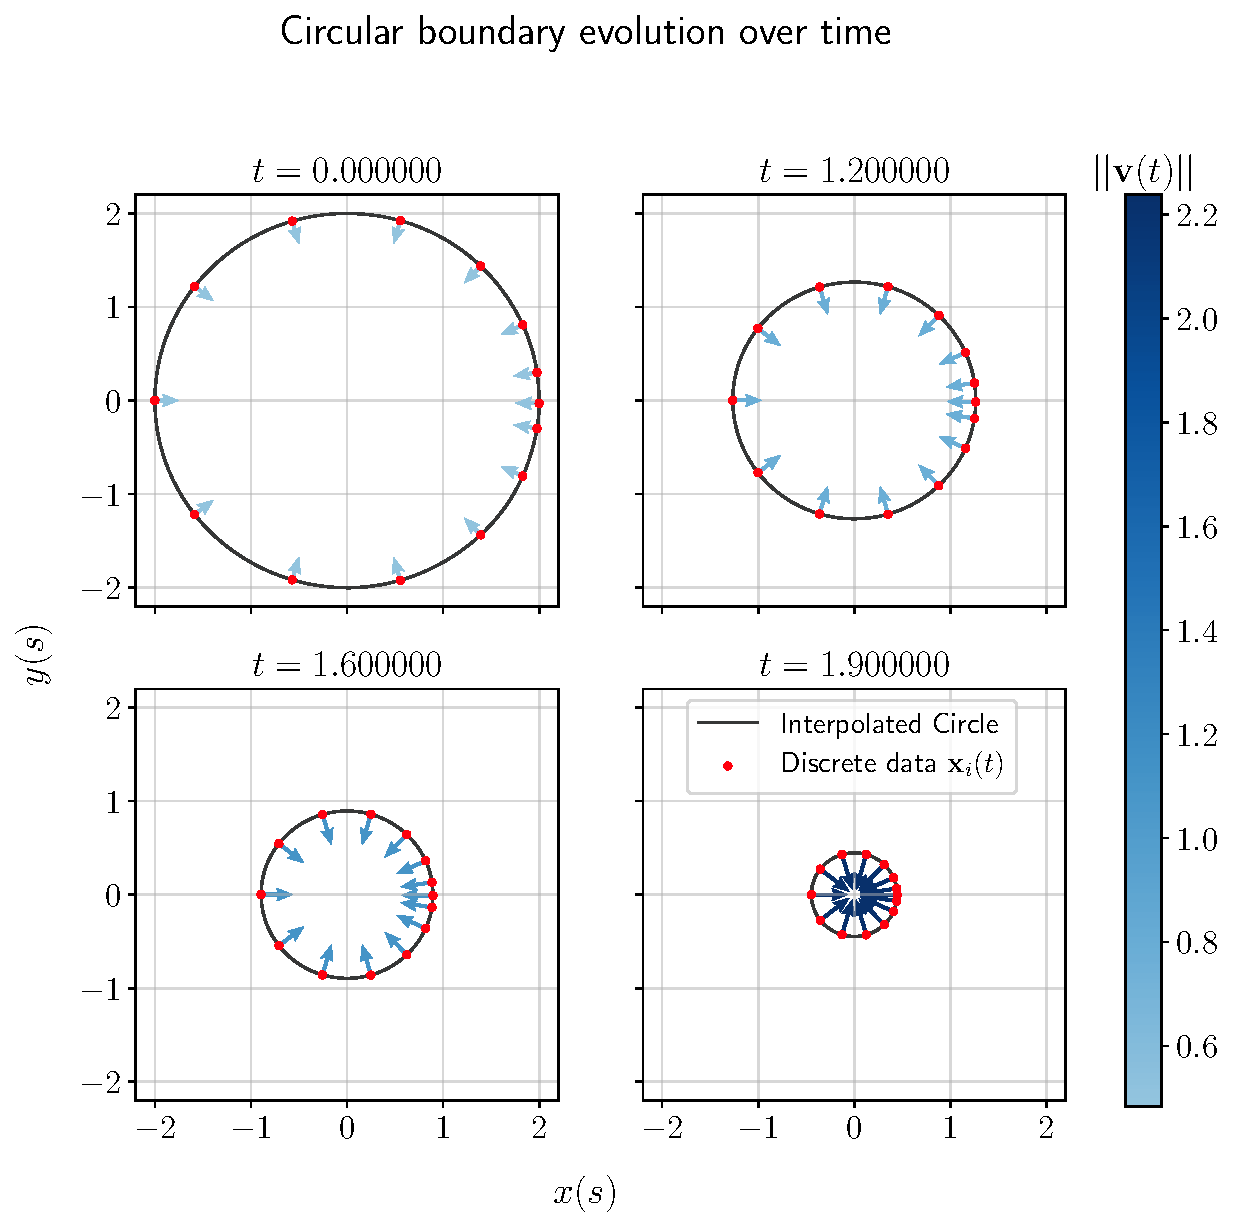
\includegraphics[scale=0.6]{circularboundary.pdf}
    \caption[Circular boundary evolution]{(Top left) The initial condition at $t=0$ of the circular boundary with $R_0 = 2$. (Top right, bottom left) After some time the circle start to shrink and the velocity of the boundary increases. (Bottom right) Near $t=2$ the circle becomes smaller and the velocity vectors increased their magnitude.}
    \label{fig:circularboundary}
\end{figure}

Figure \ref{fig:circularboundary_area} and \ref{fig:circularboundary_energy} shows relevant statistics of the experiment. Boundary area is in good agreement with the theoretical area. Area rate of change shows that whilst we should expect exactly $\dAdt = -2\pi$, we get some oscillations around this value, increasing in magnitude as simulation reaches $t_{lim}$. Actually the simulation is stopped at some time before reach $t_{lim}$, because of the mentioned acceleration of the circular boundary. The grain boundary energy under isotropic regime becomes just the perimeter of the circle $P(t) = 2\pi R(t)$. The measured energy of the simulated circle is a monotonic decrecent function in good agreement with the theoretical perimeter obtained from the radii in \eqref{eq:radii}, as well as the rate of change of the energy. 

\begin{figure}
    \centering
    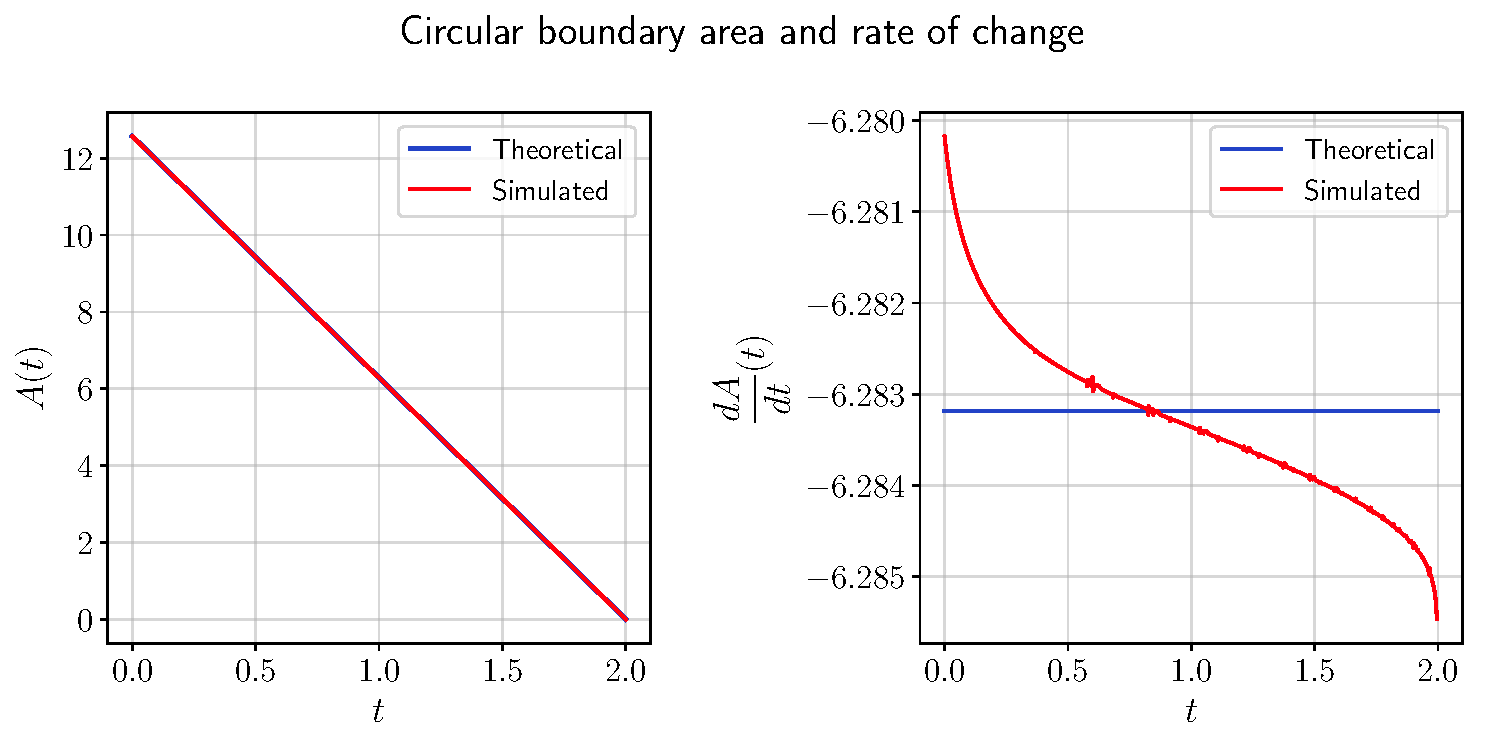
\includegraphics[scale=0.55]{circularboundary_area.pdf}
    \subfloat[\label{fig:area}]{\hspace{.55\linewidth}}
    \subfloat[\label{fig:dAdt}]{\hspace{.45\linewidth}}
    \caption[Circular boundary area and rate of change]{(a) Circle area is in good agreement with the theoretical description. (b) Rate of change is not constant in the numerical simulation, but it is near the theoretical value.}
    \label{fig:circularboundary_area}
\end{figure}

\begin{figure}
    \centering
    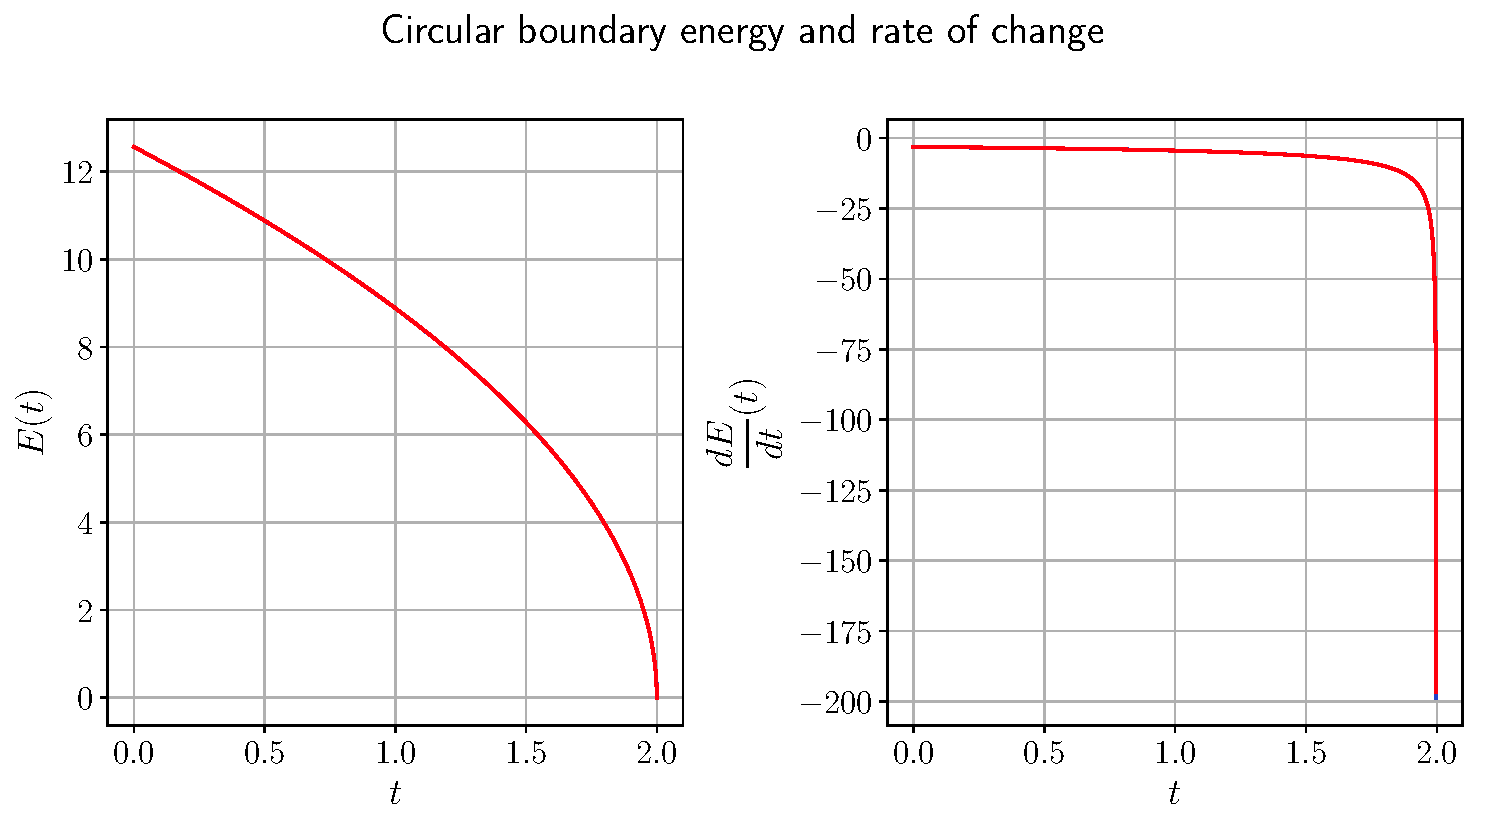
\includegraphics[scale=0.55]{circularboundary_energy.pdf}
    \subfloat[\label{fig:energy}]{\hspace{.55\linewidth}}
    \subfloat[\label{fig:dEdt}]{\hspace{.45\linewidth}}
    \caption[Circular boundary energy and rate of change]{(a) Grain energy function is in good agreement with the evolution of the perimeter of the circle. (b) rate of change of the energy, in agreement with the precipitation of the boundary motion as the radio goes to zero.}
    \label{fig:circularboundary_energy}
\end{figure}

\subsection{General Boundary}

The following example shows a boundary described by a polar rose with an initial condition:
\begin{equation*}
    \vxi(s,0) = 3 + \cos(3s)
\end{equation*}

\chapter{Grain Statistics}

In order to compare two dimensional grain arrangements with three dimensional ones, a virtual slice must be extracted from the later.
%\input{chapters/chap4.tex}
%\input{chapters/chap5.tex}
%\input{chapters/chap6.tex}
%\input{chapters/chap7.tex}
%\chapter{Conclusions}
\label{chap:conclusions}

\lettrine{T}{he} present work studied two-dimensional and three-dimensional models of grain growth and nucleation via mathematical modeling and analysis, numerical computations and statistics. Figure \ref{fig:conclusions} presents a nice overview about the topics studied in this Thesis.

% Grains topology
In relation to the grain structure this study delved into its regular topology of a graph in a torus, remarking the Euler's formula between the number of vertices $M$, boundaries $K$ and grains $N$ of the form $\displaystyle M-K+N = 0$. 
It also shows that this relation is preserved under the topological transitions of flipping and grain removal and thus along the numerical simulations of the models that was implemented.

% Closed-boundary and Coupled Model
The Coupled Model, first presented in~\cite{bachelorthesisasazo}, was improved to capture the curvature based motion and also to help the interior points - which are an abstract element for grain boundaries - to preserve the stability along the simulation. 
The curvature based motion was recovered by studying motion in regular and non-regular closed boundaries theoretically and numerically. 
This yielded that the velocity of the interior points needs a correction proportional to $1/\norm{\mylvec_i}$. 
This effectively makes small grains to be removed faster, as expected by curvature motion. 

On the other hand the interior points stability is not preserved using the vertices and interior points motion equations presented in \eqref{eq:triplejunctionsvel} and \eqref{eq:interiorpointsvel}. We developed a tangential component of the velocity that helps the interior points to move in a direction of energy minimization and also to preserve the initial equispaced positions. 
The total velocity of the interior points therefore is described by a normal component and a tangential component.
% Talk about multisteps
We also developed multisteps algorithms that helps to compute the boundaries extinction time more precisely, avoiding delays in topological transitions. Since the curvature of the boundaries may increase a lot near its collapse, the velocities of the interior points grows and the extinction time of boundaries is not reliable. In order to control the velocities and knowing a candidate steady state given by the straight line between the vertices of the boundary,  a predictor-corrector algorithm was developed to scale the velocities, stabilize the motion and prevent such growth that also delays flippings.

Numerical experiments shows that given the set of parameters that propitiate curvature motion we recover the associated statistics. 
Dihedral angles are around $2\pi/3$ and relative areas distribution shows few small grains, although it is not a log-normal distribution. 
Under anisotropic grain boundary energy, the GBCD is recovered succesfully. 
Von Neumann-Mullins relation is also approximated.

An extended Vertex Model was developed, the Continuous Stored Energy Vertex Model, which considers the introduction of an intragranular energy which allows a grain network to nucleate, that is, to create small grains and let them grow.
We analized when a nucleated grain can grow and we determined a criteria to choose a vertex to introduce the new grain such that will grow. This grain effectively adds more energy to the system, but this grain helps to energy minimization by its growth. The simulations recover successfully a stage of grain growth followed by nucleations that will eventually replace all the original grains in the system and will evolve as a grain growth model. We also tested two values of orientations for the nucleated grains, orientation zero for all grains nucleated or a local optimized orientation that minimized the added energy to the system in function of the neighbor grains. Statistics shows that the stages of grain growth and nucleation can be identified clearly, and that the GBCD is recovered and also feels the consequence of choosing certain orientation to nucleate.

% The parallel system
The Coupled Model as well as the Stored Energy Vertex Model were implemented in GPU, and efforts were directed to parallelize both models using the approach of defining the basic units of works, which ultimately were vertices and boundaries. 
Operations, such as compute boundaries velocities and move their positions, or compute vertices energies, are carried in parallel for each boundary and vertex respectively. 
A demanding task to be parallelized was the management of topological transition, a sequential algorithm that had to be posed again to be programmed in parallel to take advantage of parallelism. 
The final algorithm was the Parallel Polling System, which is essentially a fixed point iteration that ban all unsafe flippings that, when executed in parallel, lead to race conditions.

% 3d grains
Given the acquired knowledge of topological transitions in two dimensional grain growth, an extension of the Vertex Model in three dimensions was modeled with the objective of avoid topological transitions since in three dimensions they becomes more difficult to handle. 
This lead to an Implicit-transition Model~\cite{sazo2017implicit} which defines the evolution equations of the centroids of the Voronoi tessellation instead of the quadruple junctions since moving each quadruple junction by itself breaks the planar grain surfaces that represents the extension of the Vertex Model to three dimensions.
To avoid the topological transitions at each time step the new grain configuration is given by a new tessellation. 
We observed that this effectively decreases the energy asymptotically -but not monotonically, as sometimes the energy of the system increases- and we also observe the existence of continuous motion and topological transitions such as flippings, grain removals and grain surfaces becoming triple lines.

% esedoglu
A three-dimensional model was studied to obtain two-dimensional statistics. 
The model, based on mean curvature motion, was simulated and several outputs were obtained which consisted in cubes of grains with periodic boundary conditions. 
Several slices in $x$,$y$ and $z$-axis were extracted and analyzed using image analysis tools.
The results of the analysis are grain areas with units relative to the size of the image given, therefore the areas are normalized and then relative grain area distributions were obtained. 
The distribution from slices showed a tail towards small grains, which clearly deviates from a log-normal distribution and experimental data provided. 
This might be also related not by the model output itself but by the error introduced by the technique used to obtain the grain areas which required fine tuning and ignored the periodic boundary conditions.

\section{Future Work}

%The Coupled Model, as well as the Stored Energy Vertex Model, were implemented in GPU, and little time was dedicated to optimize the code for this architecture, thus it is important to perform performance profiling to this codes to identify potential bottlenecks and fix them.
The Coupled Model as well as the Stored Energy Vertex Model were implemented in GPU with CUDA. Efforts were made to reduce computation time, 
for example reducing global memory access and allocation, but there is still room for optimization for this architecture. 
It is important to obtain a performance profile of the codes in order to identify potential bottlenecks and improve the code.

The Coupled Model has the flexibility to manage more data structure related to vertices, boundaries and grains. 
For example, the introduction of stored energy and nucleation might be interesting and challenging. Nucleation sites study shall be revisited to include interior points as possible candidates sites.

Three-dimensional models inspired in the Implicit-transition Model can be developed further, for example, to look for an evolution equation of the Voronoi centroids that minimize monotonically the energy, for example the presented equation in \eqref{eq:voronoivel2} which decreases the energy monotonically during a transient state. This proposal needs to be studied further and we are currently working in this model.

The election of a $\Delta t$ for numerical simulations is still an issue since the current method to obtain stable results is to try several values. If we were able to set an optimal $\Delta t$  we would be in a good setting to automatize even more the simulations and statistics extractions. The Periodic Hausdorff Distance used in~\cite{bachelorthesismunoz} it is a good choice to analyze the convergence of the grain structure and determine $\Delta t$.


% \tikzset{%
%   >={Latex[width=2mm,length=2mm]},
%             base/.style = {rectangle, rounded corners, draw=black,
%                           minimum width=4cm, minimum height=1cm,
%                           text centered, font=\sffamily},
%   main/.style = {base, fill=RoyalBlue!30},
%   submain/.style = {base, fill=LimeGreen!50!white},
%   theme/.style = {base, minimum width=2.5cm, fill=Dandelion!40, text width=4cm},
% }
% \begin{figure}[h]
% \centering
% \begin{tikzpicture}[node distance=3cm,
%     every node/.style={fill=white, font=\sffamily}, align=center]
%   % Specification of nodes (position, etc.)
%   \node (start) [main] {Master Thesis};
  
%   \node (2dgg) [submain, below left of=start]  {2D Grain Growth};
  
%   \node (3dgg) [submain, below right of=start]  {3D Grain Growth};
  
%   \node (voronoi) [theme, below right of=3dgg]  {Implicit-transition Model: A};
  
%  \node (esedoglu) [theme, below of=voronoi]  {Extraction of Grains and Statistics};
  
%  \node (coupled) [theme, below left of=2dgg]  {Coupled Model};
 
%  \node (se) [theme, below of=coupled]  {Stored Energy Model with Nucleation};
    
    
%   % Specification of lines between nodes specified above
%   % with aditional nodes for description
%   \draw[->]             (start) -- (2dgg);
%   \draw[->]             (start) -- (3dgg);

% \end{tikzpicture}
% \caption{Overview of the topics addressed in the Thesis.}
% \label{fig:conclusions}
% \end{figure}



\bibliographystyle{abbrv}
\bibliography{References}
%
%\bibliographystyle{IEEEtran}

% --- Para los apendices
%\renewcommand{\appendixname}{Anexo}
%\renewcommand{\appendixtocname}{Anexo}
%\renewcommand{\appendixpagename}{Anexo}

%\begin{appendices}

%\input{chapters/anexo1.tex}
%\end{appendices}

\end{document}